\section{Detector Calibration}
   The gas \v{C}erenkov detector (GC) in each HRS contains 10 PMTs. The calorimeter in HRS-L contains two layers, Pion-Rejector-1 (PRL1) and Pion-Rejector-2 (PRL2), each of which has 34 PMTs. The calorimeter in HRS-R has 48 and 80 PMTs in Pre-Shower (PS) and Shower (SH), respectively. These PMTs collect the signals created by a particle passing through the detectors. The read-out signal from each PMT is split into two copies which are then recorded in the TDC and the ADC front-ends, respectively.
   
   For a common-stop TDC module, the channel numbers in the TDC spectrum represent the time difference between when the event triggers and when the STOP signal arrives. The channel numbers in the ADC spectrum, on the other hand, are directly related to the strength of the PMT signals. However, the PMT signal not only is proportional to the photon energy, but also depends on the high voltage on the PMT as well as the amplitude of the background signal. Hence, when collecting the signals with the same strength, different PMTs in the same detector may give different channel numbers in their ADC spectra. In the DB, each detector is associated with a group of parameters, or called gain factors, which can convert the channel number of each ADC spectrum into a common energy unit. These gain factors have to be calibrated each time the detector configuration is modified. After updating the gain factors in the DB and performing the new data replay, the calibrated ADC spectra can be added up together to obtain the total energy deposited by the particles in the detector.
 
\subsection{Gas \v{C}erenkov Detectors}
\begin{figure}[!ht]
  \begin{center}
    \subfloat[Before alignment]{
      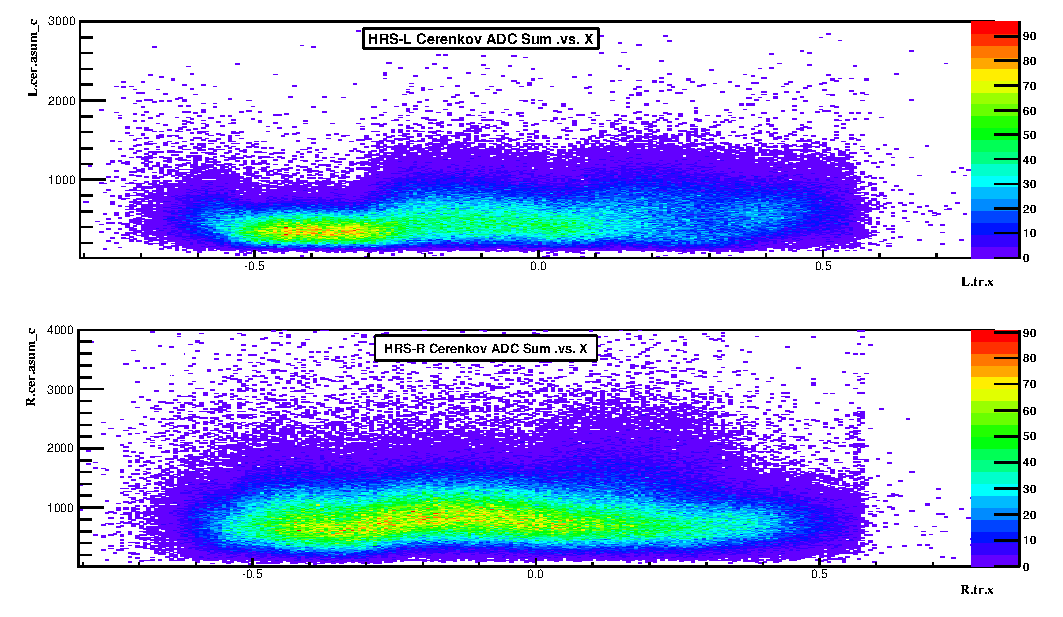
\includegraphics[type=pdf,ext=.pdf,read=.pdf,width=1.0\textwidth]{./figures/cer/Cerenkov_ADC_Align_Before}
    }
    \\ 
    \subfloat[After alignment]{
      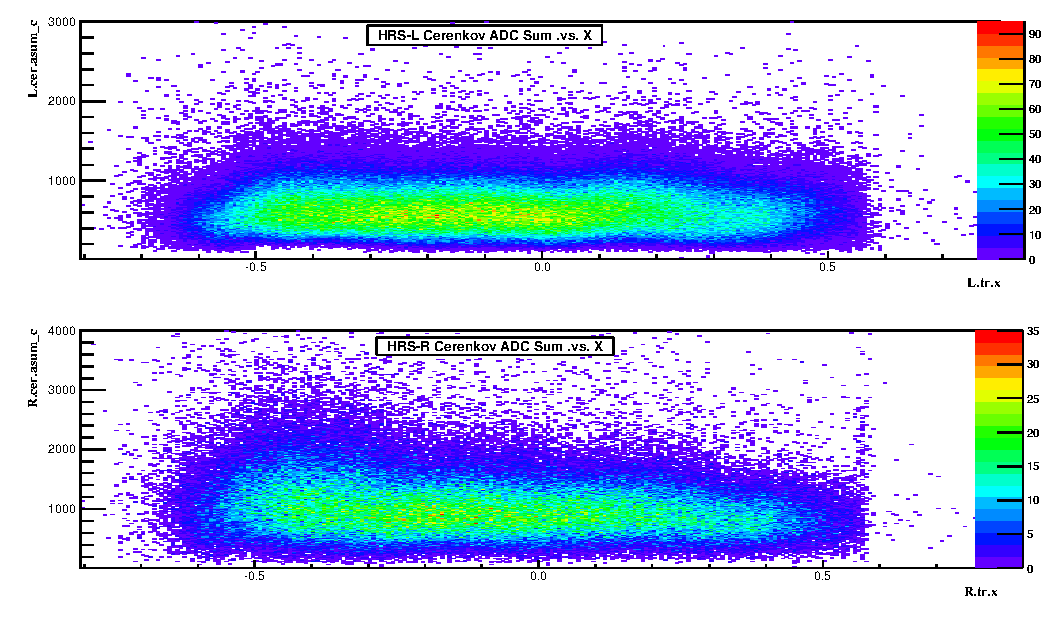
\includegraphics[type=pdf,ext=.pdf,read=.pdf,width=1.0\textwidth]{./figures/cer/Cerenkov_ADC_Align_After}
    }
    \caption[Alignment of gas \v{C}erenkov detectors]{\footnotesize{Alignment of gas \v{C}erenkov detectors (GC). Each 2-D histogram gives the distribution of the sum of the GC ADC spectra along the detector plane. Plots in (a), top for HRS-L and bottom for HRS-R, show that the ADC peaks are off by certain channels before the calibration. Plots in (b) demonstrate that those peaks are nearly at the same channel number after the alignment.}}
    \label{cer_align}
  \end{center}
\end{figure}

 The energy of a single photon which causes the emission of the single photo-electron (SPE) is only determined by the material of the photocathode in the PMT. If all PMTs for the detector are from the same model, the SPE peaks should represent the same photon energy in their ADC spectra. A calibration procedure of the GC aims to adjust the single photon electron (SPE) peak in each ADC spectrum to appear at channel 100. The gain factor for the $ith$ PMT is defined as:
\begin{equation}
  C_{i} = \frac{100}{M_{i}^{SPE}-M_{i}^{ped}},
  \label{eq_cer_gain}
\end{equation}
where $M_{i}^{SPE}$ and $M_{i}^{ped}$ are the mean values of the SPE peak and the pedestal peak in the $ith$ ADC spectrum. 
\begin{figure}[!ht]
  \begin{center}
    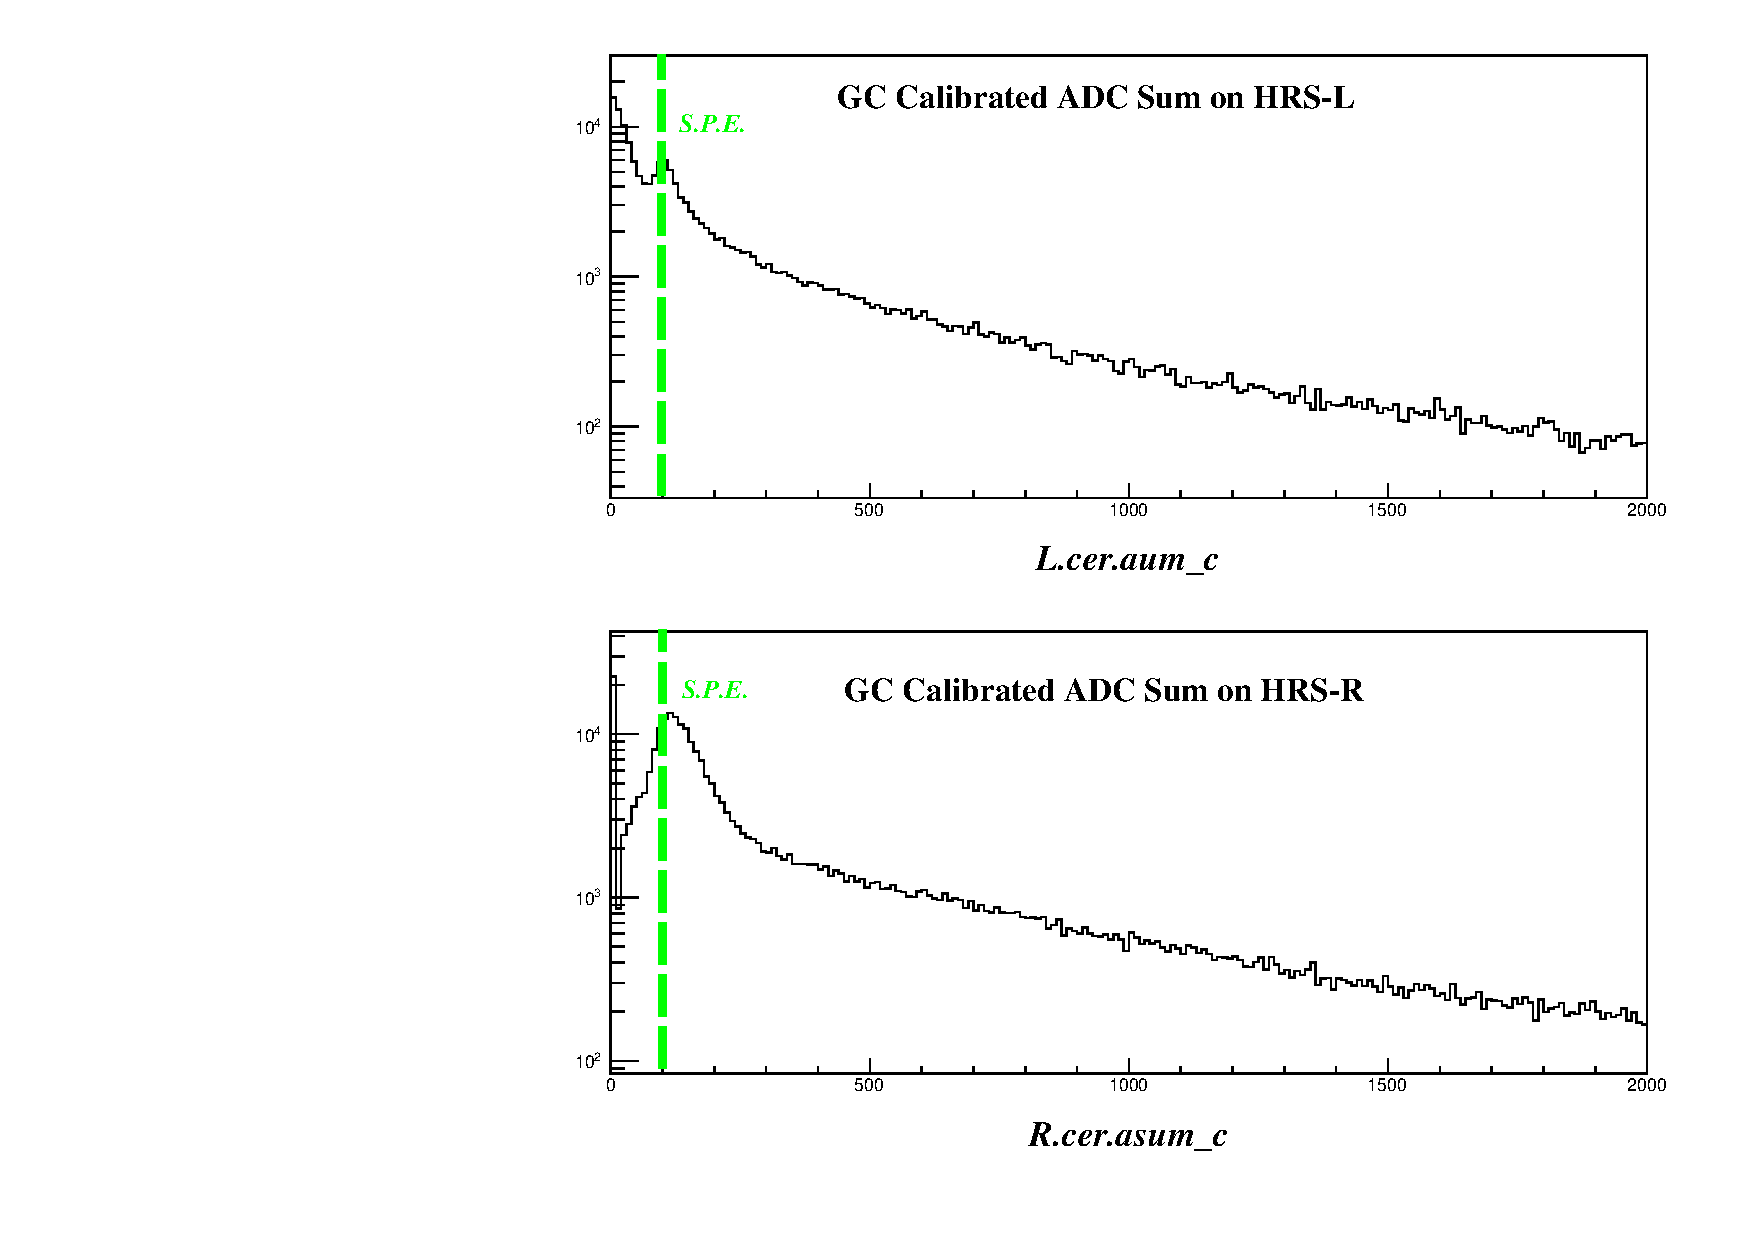
\includegraphics[type=pdf,ext=.pdf,read=.pdf,width=0.60\linewidth]{./figures/cer/Cer_SPE}
    \caption[Single electron peaks on both GCs]{\footnotesize{Single photon electron peaks (SPE) in the sum of the GC ADC spectra. Top for HRS-L and Bottom for HRS-R. The green lines indicate that the SPE peaks have been properly aligned at 100 ADC channels on each GC. (Narrow the range to 500!)}}
  \label{cer_spe}
  \end{center}
\end{figure}

 The SPE peaks didn't show on the ADC spectra when plotting events from the main production triggers (T1 for HRS-R and T3 for HRS-L). A threshold was set on the GC to form these triggers, and it excluded most of weak signals, including SPEs. The calibration was performed with events from the T6 trigger for HRS-R and the T7 trigger for HRS-L which didn't include the GCs. The raw ADC spectrum of each PMT was plotted and the channel numbers of the pedestal peak and the SPE peak were identified and recorded. The gain factors for all ten PMTs in the GC were calculated with Eq.~\eqref{eq_cer_gain} and their values were updated in the DB. The data was replayed again with these new parameters and then the calibrated ADC spectra for all PMTs had the same energy scale.
 
 Fig.~\ref{cer_align} shows that the calibrated ADC spectra were well aligned. The sum of ten calibrated ADC spectra clearly shows the SPE peak located at channel 100, as shown in Fig.~\ref{cer_spe}, and can now be directly used for the particle identification.

\subsection{Electromagnetic Calorimeters}
  The Hall-A calorimeters are able to measure the energy of few GeV electrons deposited exclusively in the detectors. The resolution of the energy measurement is determined by the design of calorimeters, as well as the energy range and the type of charge particles. In general, the energy resolution of a calorimeter can be parametrized by\cite{R_Bock}:
\begin{equation}
  \frac{\sigma(E)}{E} = a \oplus \frac{b}{\sqrt{E}},
\end{equation}
where $\oplus$ represents two terms added in quadrature. The first term is mainly contributed by systematic errors, such as intrinsic shower fluctuations, which should be small for homogeneous calorimeters, such as total absorbers. The value of second term is determined by the uniformity of calorimeters as well as uncertainty of detector calibration. It is typically $\mathrm{5\%/\sqrt{E}}$ for lead glass calorimeters. 

  The electron creates a track during the cascade and the lead glass blocks along the track collect these photon signals. During the data replay, these blocks can be identified by using the VDC tracking information, and within the same layer the group of these blocks is called a cluster. The sum of their ADC spectra after the calibration denotes the energy deposited in this cluster, and should be distinguished from the sum of all calibrated ADC spectra since blocks outside the cluster only pick up the background signals. Once the individual ADC spectra are calibrated, the sum of the energy deposited in both layers should be equal to the energy (or equivalently the momentum) of scattered electrons. A new variable, E/P, is defined as the ratio of the energy sum of two clusters to the electron's momentum, and should be centered at one if the gain factors are properly calibrated. Different procedures were applied on each calorimeter. 
 
 \begin{figure}[!ht]
  \begin{center}
     \subfloat[Pion Rejectors on HRS-L]{
      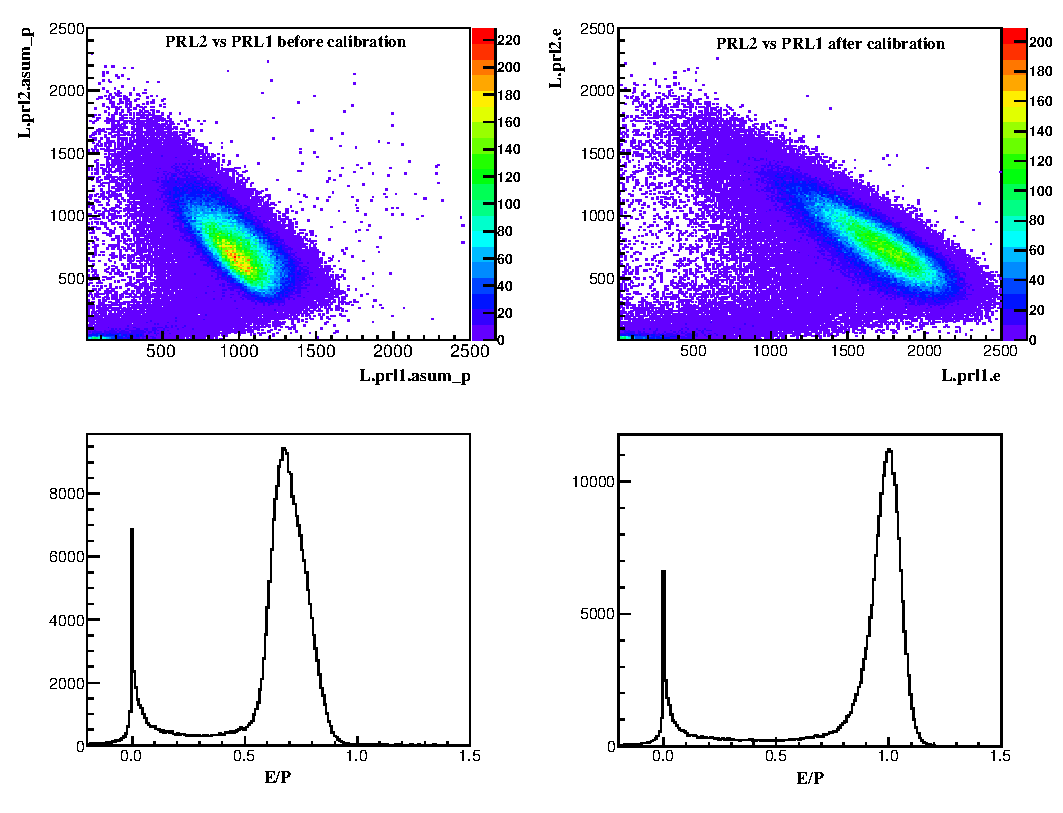
\includegraphics[type=pdf,ext=.pdf,read=.pdf,width=0.75\linewidth]{./figures/calo/PRL_Calibration}
      \label{prl_cali}
   }
   \\
    \subfloat[Pre-Shower and Shower on HRS-R]{
      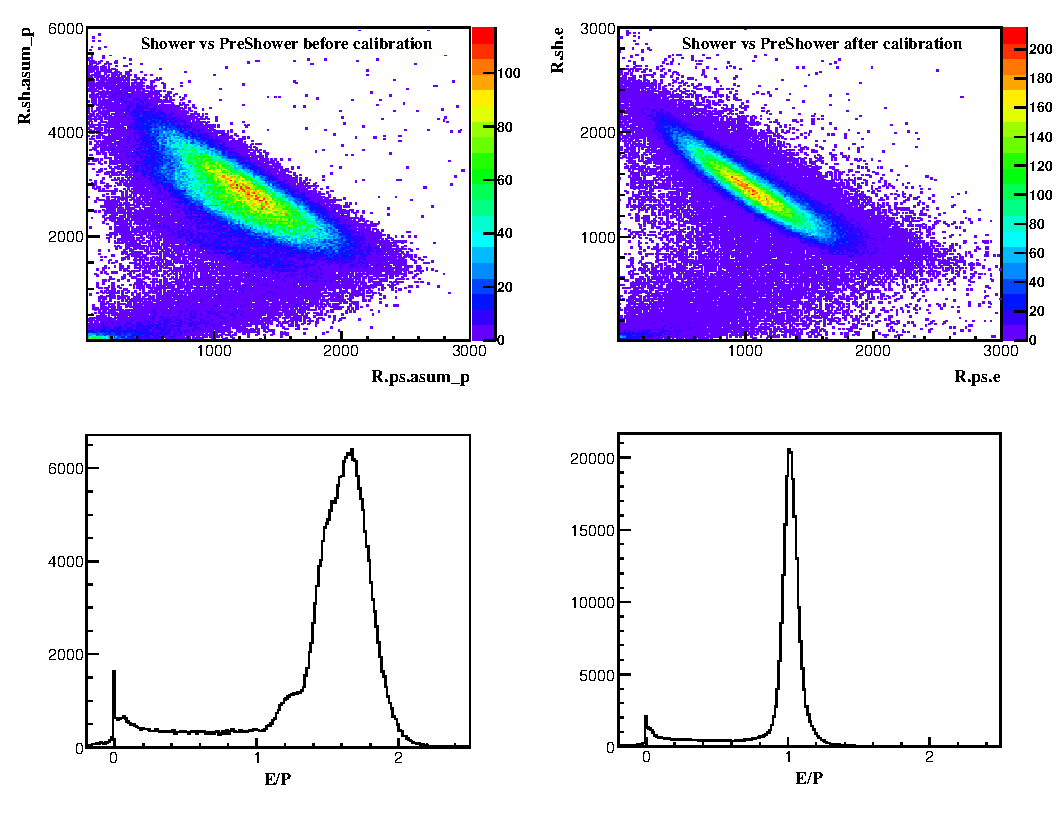
\includegraphics[type=pdf,ext=.pdf,read=.pdf,width=0.75\linewidth]{./figures/calo/SH_Calibration}
      \label{sh_cali}
      }
   \caption[Calibration of calorimeters]{\footnotesize{Calibration of calorimeters. In each figure, the top two plots are the 2-D histograms of the PRL1 (PS) ADC sum versus the PRL2 (SH) ADC sum before and after the calibration. The electron band is clearly isolated after the calibration. The bottom two 1-D histograms are the distributions of E/P before and after the calibration. The peak becomes sharp and locates at one with new gain factors.}}
   \label{calo_cali}
  \end{center}
\end{figure}
 A minimization method was used to calibrate the calorimeter on HRS-R, composed of two layers, Pre-Shower (PS) and Shower (SH)\cite{shower_ak}. The Chi-Square was defined as: 
\begin{equation}
  \chi^{2} = \sum_{i=1}^{N}\left[\sum_{j\in M_{ps}^{i}}C_{j}\cdot (ADC_{j}^{i}-Ped_{j})+\sum_{k\in M_{sh}^{i}}C_{k}\cdot (ADC_{k}^{i}-Ped_{k})-P_{kin}^{i}\right]^{2},
\end{equation}
where \emph{i} is the \emph{ith} event; \emph{j} is the \emph{jth} PS block; \emph{k} is the \emph{kth} SH block; $M_{ps}^{i}$ and $M_{sh}^{i}$ are sets of PS and SH blocks included in the reconstructed cluster for the \emph{ith} event; $ADC_{j/k}^{i}$ and $Ped_{j/k}$ represent the ADC channel number of the event and mean pedestal value in the ADC spectrum, respectively; $P_{kin}^{i}$ is the particle momentum of the \emph{ith} event; and $C_{j/k}$ is the gain factor of the ADC spectrum used as a fitting parameter during the minimization.

 To obtain the best fitting result, electron samples were selected from data taken in the QE tail ($x_{bj}>1$) where scattered electrons were uniformly distributed among all lead glass blocks. A minimization package \cite{shower_luhj} was called to minimize $\chi^{2}$, and the gain factors obtained from the fitting parameters were stored in the database.

  The calorimeter on HRS-L, composed of the layers of Pion-Rejector-1 (PRL1) and Pion-Rejector-2 (PRL2), is not a total absorber and the minimization method used on the PS and SH is not applicable. Instead, it was calibrated by aligning the minimum ionization peak of each ADC spectrum to a common channel number, similar to the GC calibration. The cosmic ray events were used during the calibration since they were uniformly distributed along the entire blocks. Furthermore, the particles in cosmic ray are mostly muons which have small energy spread. The pedestal peak ($ADC_{i}^{ped}$) and muon peak ($ADC_{i}^{muon}$) in the ADC spectrum of the $ith$ PMT were located and their distance were aligned to 100, by applying a gain factor defined as:
\begin{equation}
  C_{i} = \frac{100}{ADC_{i}^{muon}-ADC_{i}^{ped}}.
\end{equation}
 The gain factors for all PMTs in PRL1 and PRL2 were calculated similarly. With these updated gain factors in the data base, the E/P was calculated at the new data replay. To shift the peak of the E/P distribution to one, the gain factors were further adjusted:
\begin{equation}
  C_{i}^{real} = C_{i} \times \frac{1}{M_{E/P}},
\end{equation}
where $M_{E/P}$ represents the mean value of the E/P peak before the adjustment. The adjusted gain factors were then updated in the data base and the data was replayed again.
\begin{figure}[!ht]
  \begin{center}
    \subfloat[on HRS-L]{
      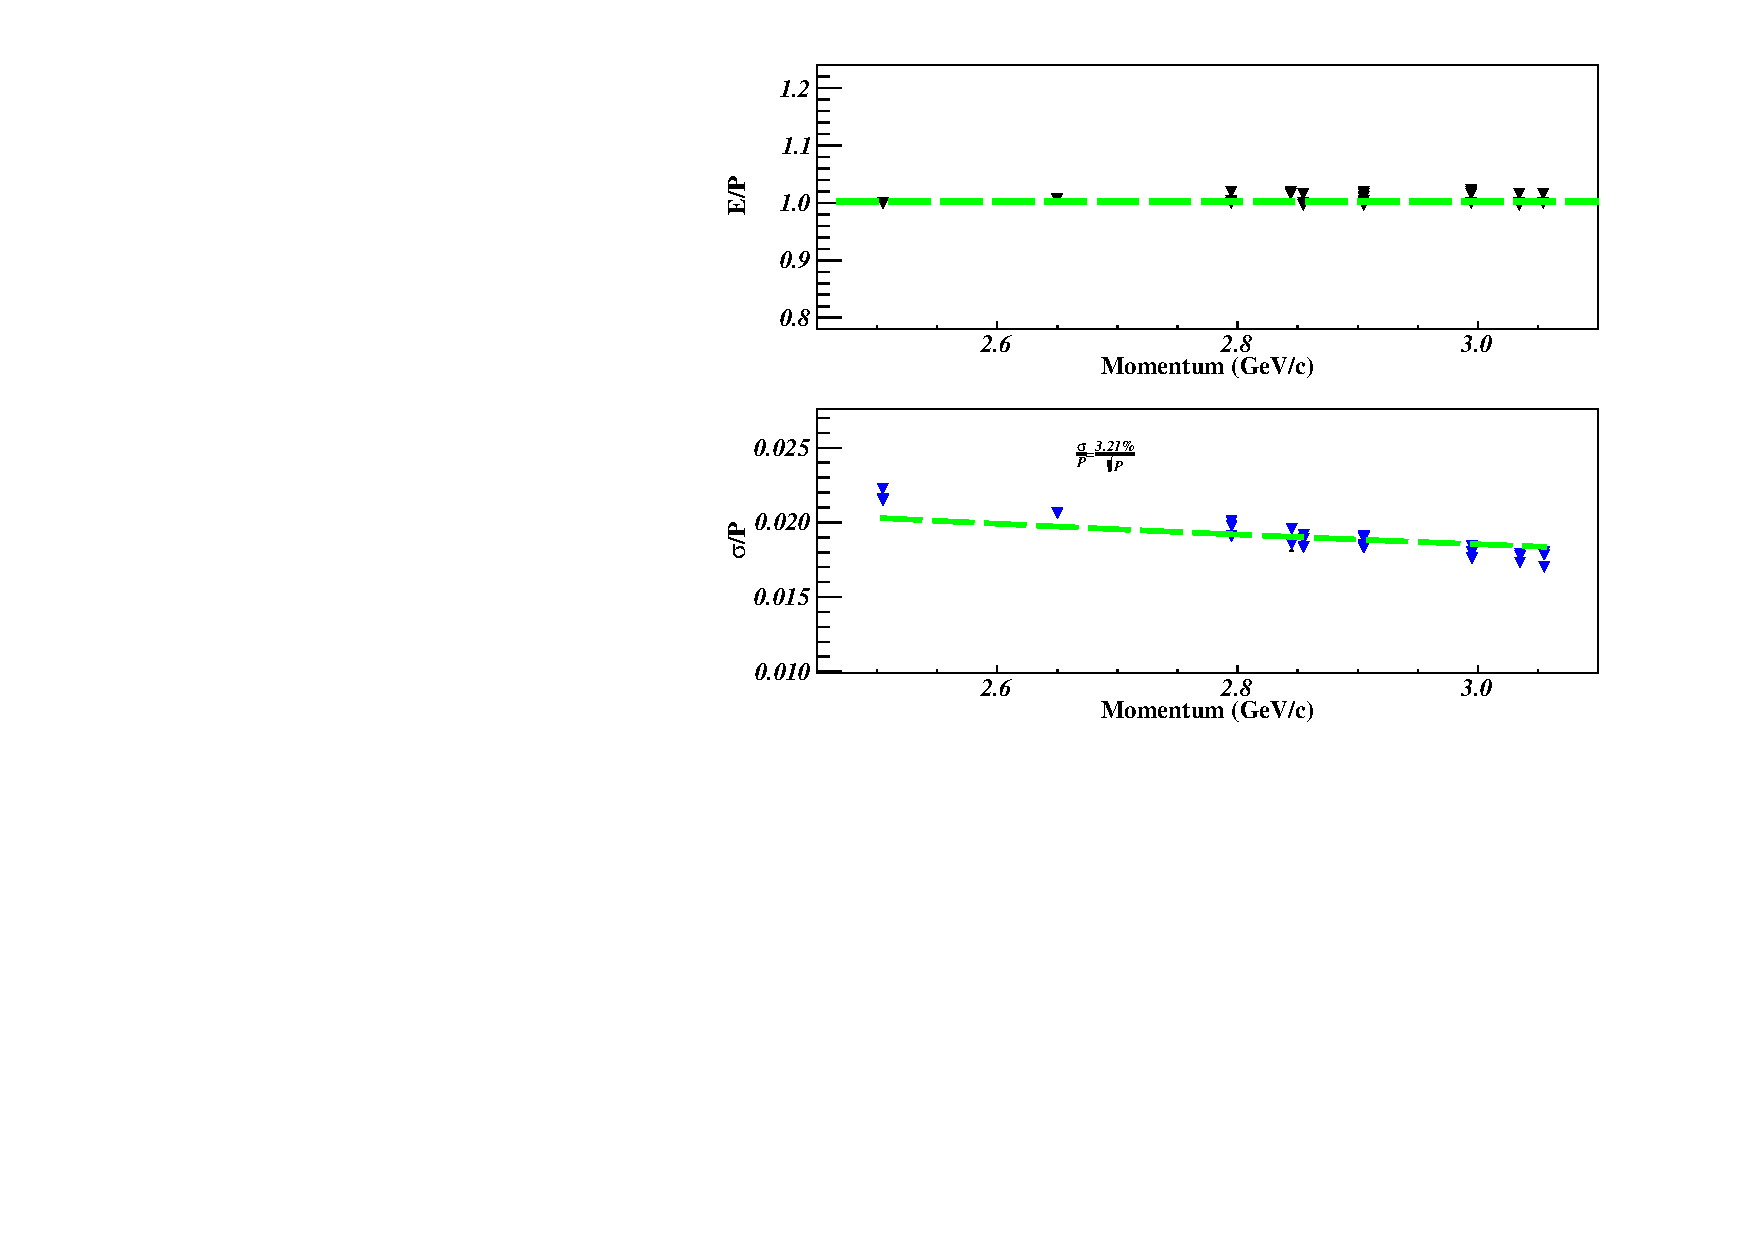
\includegraphics[type=pdf,ext=.pdf,read=.pdf,width=0.9\textwidth]{./figures/calo/L_Calo_Align_new}
    }
    \\ 
    \subfloat[on HRS-R]{
      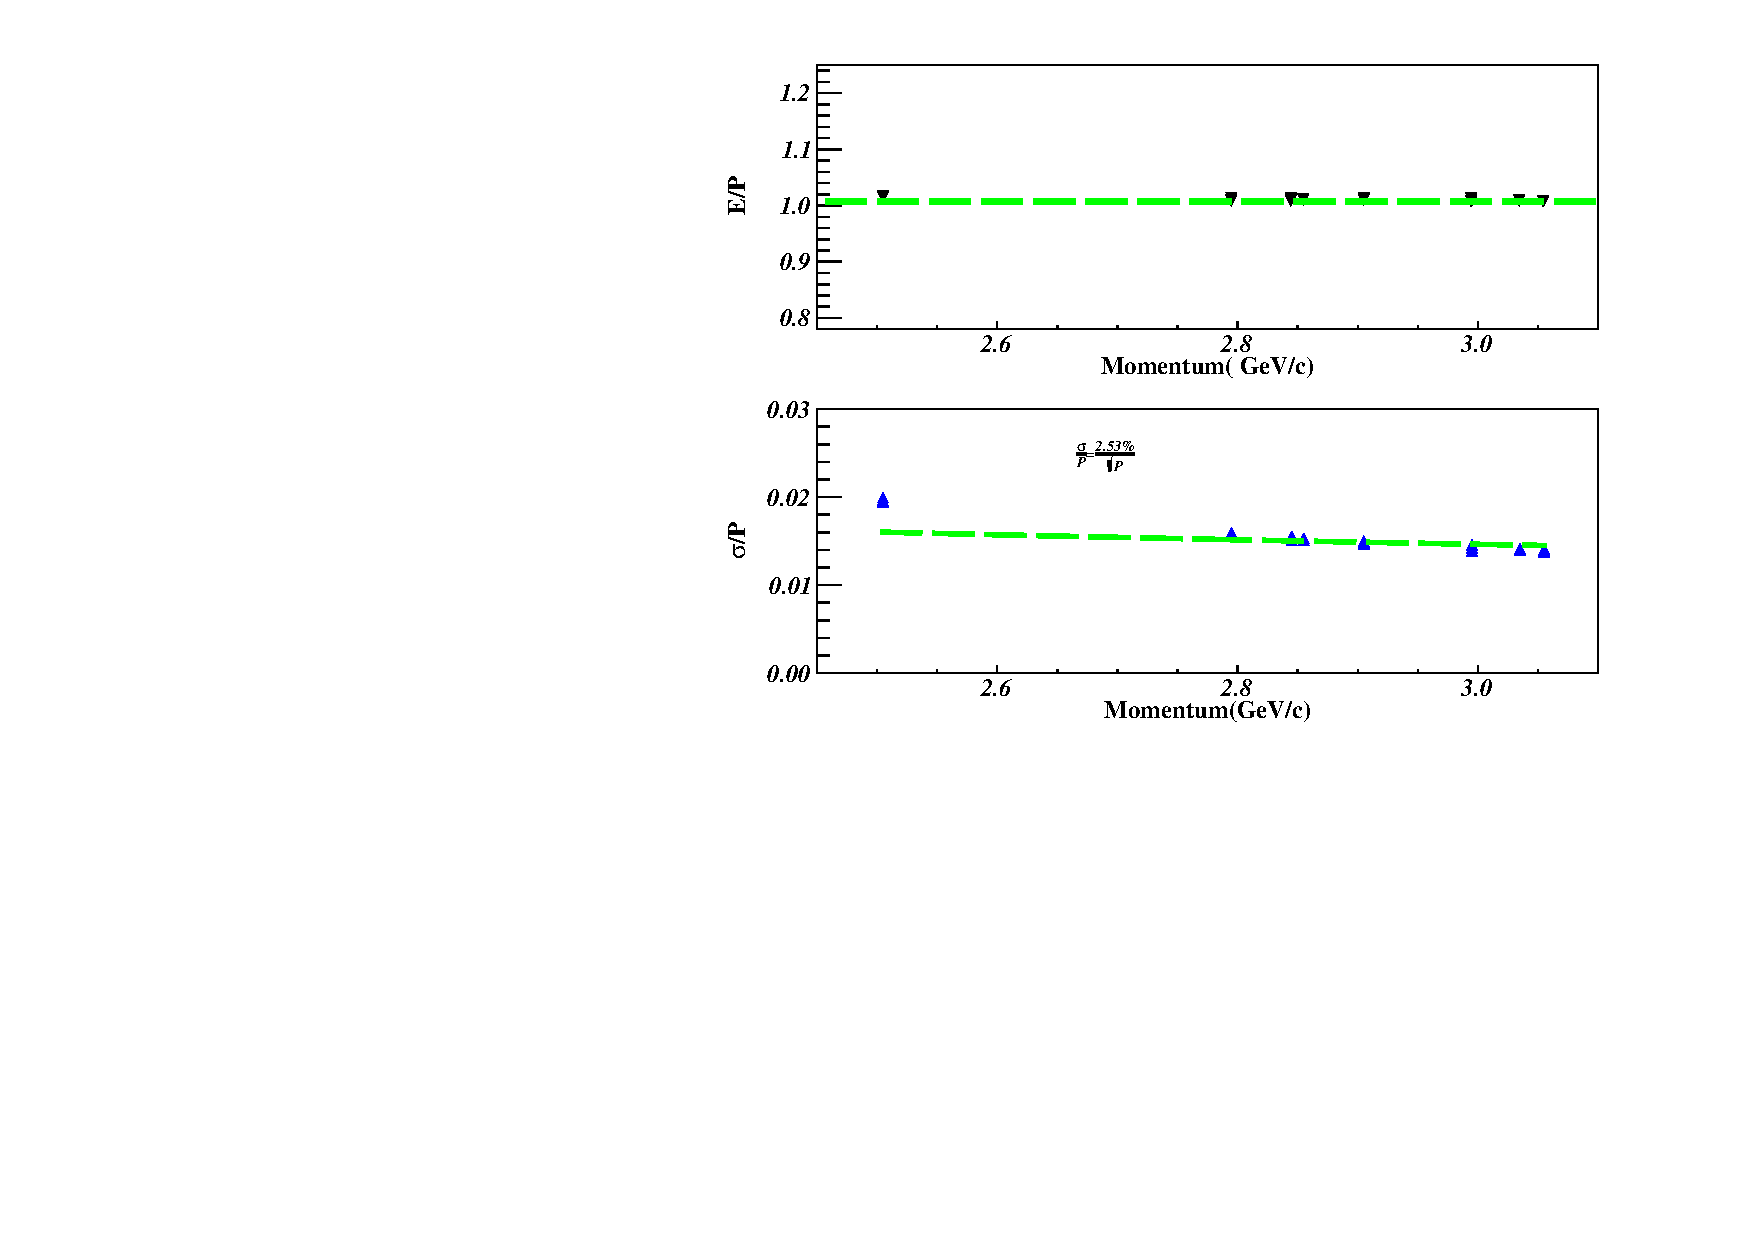
\includegraphics[type=pdf,ext=.pdf,read=.pdf,width=0.9\textwidth]{./figures/calo/R_Calo_Align_new}
    }
    \caption[Calibration performance and resolution of calorimeters]{\footnotesize{Calibration performance and resolution of calorimeters. The top plot in each figure reveals the performance of calibration at different momentum setting. The two bottom plots give the resolution of calorimeters, which are 3.21\%$\mathrm{/\sqrt{GeV}}$ on HRS-L and 2.53\%$\mathrm{/\sqrt{GeV}}$ on HRS-R.} }
    \label{calo_resol}
  \end{center}
\end{figure}

 The calibration results of both calorimeters are shown in Fig.~\ref{calo_cali}, where electrons are better separated from backgrounds and E/P is well centered at one. The locations of E/P peaks at different momentum settings are shown in Fig.~\ref{calo_resol}. The energy resolution was also given by fitting the spread of \emph{E/P} peaks as the function of the momentum. The overall resolution of PS and SH is 2.53\%$\mathrm{/\sqrt{GeV}}$. The resolution of Pion Rejectors is 3.21\%$/\mathrm{\sqrt{GeV}}$, slightly worse as they are not total absorbers.